\subsection{Testprotokoll zu /LF05/ Wiedergabe über Audio Codec}
\label{test-audiocodec}

\textbf{\hyperlink{lf-audioplayback}{LF05}}

\paragraph{Ziel:}
Überprüfung der Grundfunktionalität und Ansteuerung des Audio Codecs.

\paragraph{Durchführung:}

Um Grundfunktionalität des Audio Codecs sicherstellen, wird die Audiowiedergabe ohne die Verwendung von Dateizugriffen von der SD-Karte durchgeführt. 
Somit wird eine mögliche Fehlerquelle eliminiert, was die Fehlersuche deutlich vereinfacht. 
Die Audiodaten, in Form einer Sinuswelle, werden in einen Lookup-Table generiert. 

\inputminted[firstline=15, lastline=19]{c}{../../f401_sd_card_audio_codec_test/Core/Src/audio.c}

Dieser Lookup-Table wird dann iterativ ausgelesen und mit folgender Funktion in den Audiobuffer geschrieben.

\inputminted[firstline=55, lastline=77]{c}{../../f401_sd_card_audio_codec_test/Core/Src/audio.c}

\newpage
\paragraph{Schritte:}
\begin{enumerate}
	\item System gemäß dem Schaltplan verbinden, wobei der Audio Codec und die Lautsprecher verbunden sind.
	\item Sinuswelle per Lookup Table Generieren. 
	\item Wiedergabe der Sinuswelle über den Audio Codec.
	\item Anschluss von Oszilloskop-Sonde mit dem Audioausgang.
	\item Visuelle Analyse der Wellenform über Oszilloskop
	\item Auditive Analyse der Sinuswelle über den Lautsprecher.
\end{enumerate}

\paragraph{Erwartete Werte:}
\begin{itemize}
	\item Die Sinuswelle sollte im Oszilloskop klar und sauber dargestellt werden.
	\item Die Audioausgabe sollte frei von Störgeräuschen wie Knacken oder Verzerrungen sein.
	\item Die Sinuswelle sollte auditiv klar und konsistent über die Lautsprecher wiedergegeben werden.
\end{itemize}

\paragraph{Testergebnisse:}
\begin{itemize}
	\item Oszilloskop zeigt eine saubere Sinuswelle ohne Verzerrungen.
	\item Die Audioausgabe ist frei von Störgeräuschen.
	\item Die Sinuswelle klingt sauber und klar über die Lautsprecher.
\end{itemize}

\begin{figure}[H]
	\centering
	\begin{subcaptionblock}{0.49\textwidth}
		\centering
		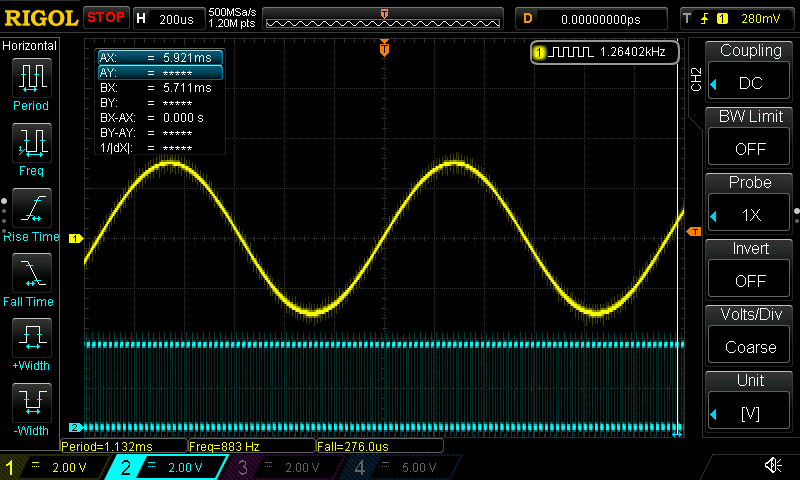
\includegraphics[width=\textwidth]{images/10_test_validierung/audio/PCM5102a-sine-double_buffer-1kHz-false.png}
		\caption{Oszilloskopansicht der Sinuswellenwiedergabe}
		\label{fig:sinuswave-test}
	\end{subcaptionblock}
	\hfill
	\begin{subcaptionblock}{0.49\textwidth}
		\centering
		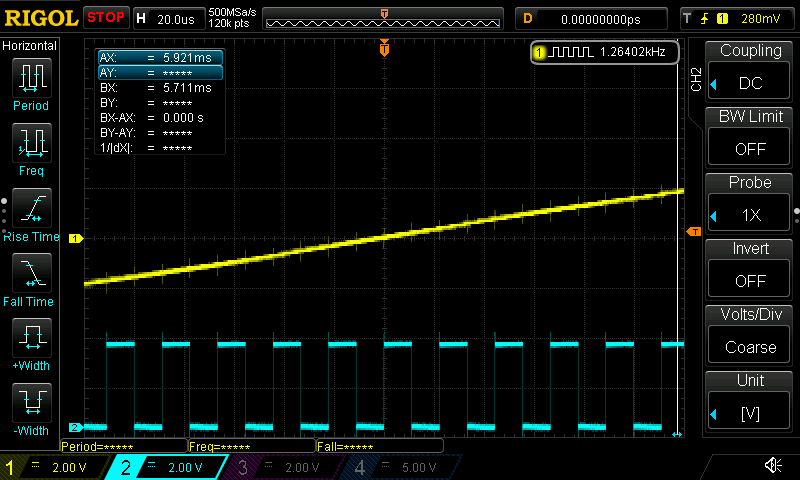
\includegraphics[width=\textwidth]{images/10_test_validierung/audio/PCM5102a-sine-double_buffer-1kHz-false-LCK.png}
		\caption{Nahe Oszilloskopansicht der Sinuswellenwiedergabe}
		\label{fig:sinuswave-test-closeup}
	\end{subcaptionblock}
\end{figure}

Die Tests des Pitchfaktors zeigen, dass die Sinuswellenwiedergabe bei allen getesteten Werten sauber und klar ist. Kleinere Abweichungen von den erwarteten Frequenzen sind vorhanden, beeinflussen jedoch nicht die Audioqualität. Die Wiedergabe bleibt störungsfrei und konsistent über die getesteten Pitchfaktoren hinweg.

\newpage
\subsection{Testprotokoll zu /LF06/ Pitchgenauigkeit des Wiedergabealgorithmus}
\label{test-pitchgenauigkeit}

\textbf{\hyperlink{lf-pitchaudio}{LF06}}

\paragraph{Ziel:}
Überprüfung der Pitchgenauigkeit des Wiedergabealgorithmus.

\paragraph{Durchführung:}

Um die Pitchgenauigkeit des Wiedergabealgorithmus zu überprüfen, wird ein \SI{440}{\hertz} Audiofile mit verschiedenen Tonhöhen über den Wiedergabealgorithmus abgespielt.

Der Pitchfaktor, also der Faktor um den die Wiedergabe verschnellert/verlangsamt wird, soll nicht über eine externen Potentiometer oder ähnlicher Hardware gesteuert werden, um unpräzise Werte zu vermeiden.
Er im folgender Funktion mit \mintinline{c}|player->pitchFactor = 2.0f;| präzise festgelegt (hardcoded):

\inputminted[firstline=15, lastline=23]{c}{../../f401_sd_card_audio_codec_test/Core/Src/wavPlayer.c}

\paragraph{Schritte:}
\begin{enumerate}
	\item System gemäß dem Schaltplan verbinden, wobei der Audio Codec und die Lautsprecher verbunden sind.
	\item Anschluss von Oszilloskop-Sonde mit dem Audioausgang.
	\item Pitchfactor auf \mintinline{c}|1.0f| setzen.
	\item Wiedergabe des \SI{440}{\hertz} Testfile über den Audio Codec.
	\item Visuelle Analyse der Wellenform über Oszilloskop (Messung der Frequenz). 
	\item Auditive Analyse der Sinuswelle über den Lautsprecher.
	
	\item Pitchfactor auf \mintinline{c}|0.5f| setzen.
	\item Wiedergabe des \SI{440}{\hertz} Testfile über den Audio Codec.
	\item Visuelle Analyse der Wellenform über Oszilloskop (Messung der Frequenz). 
	\item Auditive Analyse der Sinuswelle über den Lautsprecher.
	
	\item Pitchfactor auf \mintinline{c}|2.0f| setzen.
	\item Wiedergabe des \SI{440}{\hertz} Testfile über den Audio Codec.
	\item Visuelle Analyse der Wellenform über Oszilloskop (Messung der Frequenz). 
	\item Auditive Analyse der Sinuswelle über den Lautsprecher.
\end{enumerate}

\paragraph{Erwartete Werte:}
\begin{itemize}
	\item Die Sinuswelle sollte im Oszilloskop mit jedem Pitchfaktor klar und sauber dargestellt werden.
	\item Die Audioausgabe sollte frei von Störgeräuschen wie Knacken oder Verzerrungen sein.
	\item Die Sinuswelle sollte auditiv klar und konsistent über die Lautsprecher wiedergegeben werden.
	\item Die erwartete Frequenzen sind:
		 \begin{itemize}
		 	\item Pitchfaktor = 1.0 \(\rightarrow\) \SI{440}{\hertz}
		 	\item Pitchfaktor = 0.5 \(\rightarrow\) \SI{220}{\hertz}
		 	\item Pitchfaktor = 2.0 \(\rightarrow\) \SI{880}{\hertz}
		 \end{itemize}
\end{itemize}

\paragraph{Testergebnisse:}
\begin{itemize}
	\item Bei einem Pitchfaktor von 1.0 beträgt die gemessene Frequenz \SI{450}{\hertz} anstelle der erwarteten \SI{440}{\hertz}. 
	Abgesehen von dieser Abweichung zeigt die Sinuswelle eine klare und saubere Darstellung im Oszilloskop, und die Audioausgabe ist frei von Störgeräuschen. 
	Die Sinuswelle wird auditiv klar und konsistent über die Lautsprecher wiedergegeben.
	
	\item Bei einem Pitchfaktor von 0.5 beträgt die gemessene Frequenz \SI{225}{\hertz} anstelle der erwarteten \SI{220}{\hertz}. 
	Die Frequenz ist wie erwartet, halb so groß wie bei einem Pitchfaktor von 1.0, allerdings zeigen sich kleine Spitzen in der Wellenform auf dem Oszilloskop, die jedoch nicht hörbar sind. 
	
	
	
	\item Bei einem Pitchfaktor von 2.0 beträgt die gemessene Frequenz \SI{890}{\hertz} anstelle der erwarteten \SI{880}{\hertz}. 
	Die Frequenz ist wie erwartet, doppelt so groß wie bei einem Pitchfaktor von 1.0.
	Abgesehen von dieser Abweichung zeigt die Sinuswelle eine klare und saubere Darstellung im Oszilloskop, und die Audioausgabe ist frei von Störgeräuschen. 
	Die Sinuswelle klingt sauber und klar über die Lautsprecher.
\end{itemize}

\begin{figure}[H]
	\centering
	\begin{minipage}[b]{0.49\textwidth}
		\centering
		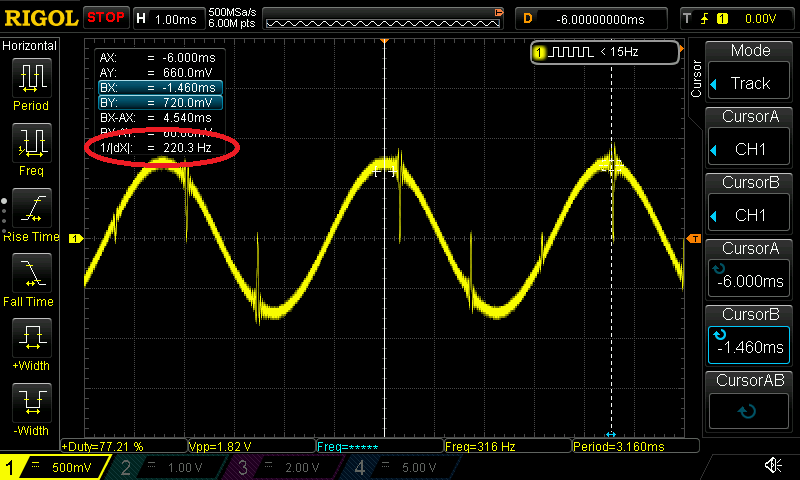
\includegraphics[width=\textwidth]{images/10_test_validierung/audio/440Hz-pitch_0.5.png}
		\caption{Frequenzmessung bei Pitchfaktor 0.5}
		\label{fig:440Hz-pitch_0.5}
	\end{minipage}
	\hfill
	\begin{minipage}[b]{0.49\textwidth}
		\centering
		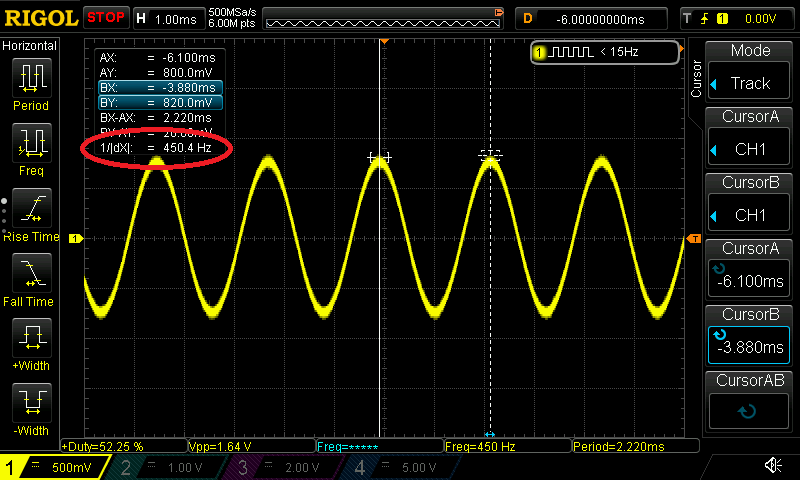
\includegraphics[width=\textwidth]{images/10_test_validierung/audio/440Hz-pitch_1.0.png}
		\caption{Frequenzmessung bei Pitchfaktor 1.0}
		\label{fig:440Hz-pitch_1.0}
	\end{minipage}
	
	\vspace{1em}
	
	\begin{minipage}[b]{0.49\textwidth}
		\centering
		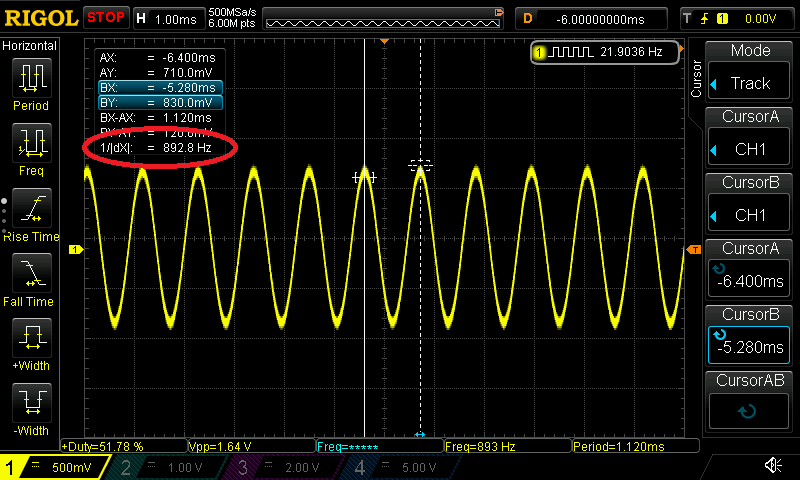
\includegraphics[width=\textwidth]{images/10_test_validierung/audio/440Hz-pitch_2.0.png}
		\caption{Frequenzmessung bei Pitchfaktor 2.0}
		\label{fig:440Hz-pitch_2.0}
	\end{minipage}
\end{figure}
\label{fig:frequenzmessung-pitch}

Die Grundfunktionalität und Ansteuerung des Audio Codecs ist sichergestellt. Die Sinuswellenwiedergabe erfolgt sauber und klar, sowohl visuell als auch auditiv, was auf eine erfolgreiche Integration und Funktionsweise des Audio Codecs hinweist.

\newpage
\subsection{Testprotokoll zu /LQ01/ Latenzmessung}
\label{test-latenzmessung}

\textbf{\hyperlink{lq-latency}{LQ01}}

Messung der Latenz vom Zeitpunkt des Triggerinputs bis zur Audioausgabe über den Audio-Codec.

Durchführung mit dem STM32-Audioprojekt aus dem Repository (\href{run:../../f401_sd_card_audio_codec_test/}{\texttt{/f401\_sd\_card\_audio\_codec\_test/}}).
Der Audio-Codec, sowie der SD-Kartenleser müssen wie im Schaltplan \ref{sec:test-schematics} verbunden werden.

\begin{minipage}{\textwidth}
\paragraph{Schritte:}
\begin{enumerate}
	\item Anschluss zweier Oszilloskop-Sonden: an Trigger-Input/Play-Button-Pin und Audio-Ausgang.
	\item Laden einer Test PCM .wav-Datei mit einer Samplerate von \SI{44.1}{\kilo\hertz}, 16 Bit und Stereo/2 Kanälen auf die SD-Karte.
	\item Umschalten des Oszilloskops in den Single-Shot-Modus und Konfiguration zur Auslösung durch den Audio-Kanal.
	\item Abspielen der Testdatei durch Auslösen des Play-Buttons.
	\item Positionierung zweier Mess-Cursor: einer auf die erste Flanke des Trigger-Input-Signals und der andere auf den Beginn des Audio-Ausgangssignals.
\end{enumerate}
\end{minipage}


\paragraph{Erwartete Werte}
	Die erwartete Latenz errechnet sich wie folgt:
	
	\textit{Gegeben:}
	\begin{align*}
		\text{Samplerate} &= \SI{44.1}{\kilo\hertz} = 44{,}100 \, \text{Samples pro Sekunde} \\
		\text{Puffergröße} &= 256 \, \text{Samples}
	\end{align*}
	
	\textit{Berechnung der Latenz:}
	
	\[
	\text{Zeit pro Sample} = \frac{1 \, \text{Sekunde}}{44{,}100 \, \text{Samples}} \approx \SI{22.68}{\micro\second}
	\]
	
	\[
	\text{Zeit für einen Puffer} = 256 \, \text{Samples} \times \SI{22.68}{\micro\second} \approx \SI{5.8}{\milli\second}
	\]
	
	Die Latenz für das System mit den angegebenen Parametern beträgt also im Idealfall \( \SI{5.8}{\milli\second} \).
	
\paragraph{Testergebnisse}

\begin{itemize}
	\item Gemessene Latenz von \SI{6.4}{\milli\second} (\textbf{BX-AX} in Abbildung  \ref{fig:audio-latency-test}).
	\item Die Abweichung von der erwarteten Latenz ist wahrscheinlich auf die Verarbeitungszeiten des Audio-Codecs zurückzuführen.
	\item Sehr praktikabler Latenzwert für Audioinstrument.
\end{itemize}

\begin{figure}[H]
	\centering
	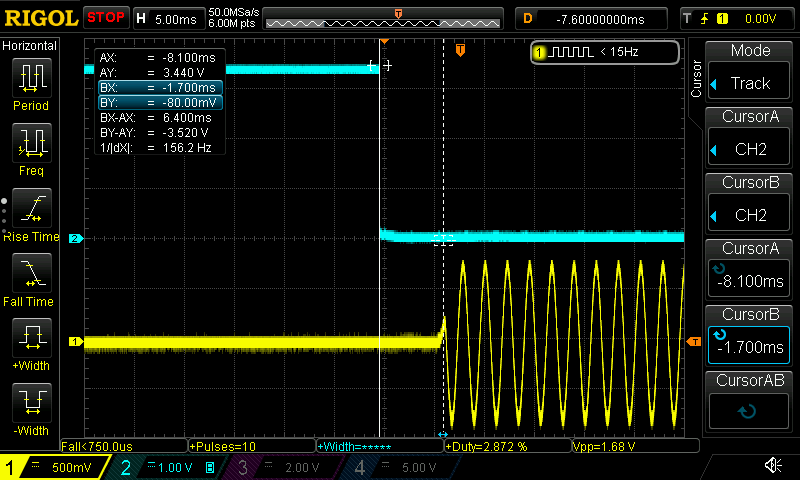
\includegraphics[width=0.6\textwidth]{images/10_test_validierung/audio/audio-latency-test.png}
	\caption{Oszilloskopansicht der Latenzmessung von Trigger (Blau) bis Audioausgang (Gelb)}
	\label{fig:audio-latency-test}
\end{figure}
